
The quench measurements have been conducted for $I=86~\text{A}$ which is a lower value than the nominal operating current of the skew quadrupole ($I=182~\text{A}$). During the test, the quench has been initiated by discharging a capacitor in series with a 2x2 $\text{mm}^2$ heater attached to the external grounding insulation of the magnet. The voltage drop across the capacitor is presented in Fig. \ref{fig:resistor_voltage_discharge_curve}. By considering the discharge curve as the \nth{1} order, one can deduce the time constant and the resistance of the heater. The obtained data are presented in Table \ref{table:heater_characteristics}.

\begin{figure}[ht!]
    \centering
    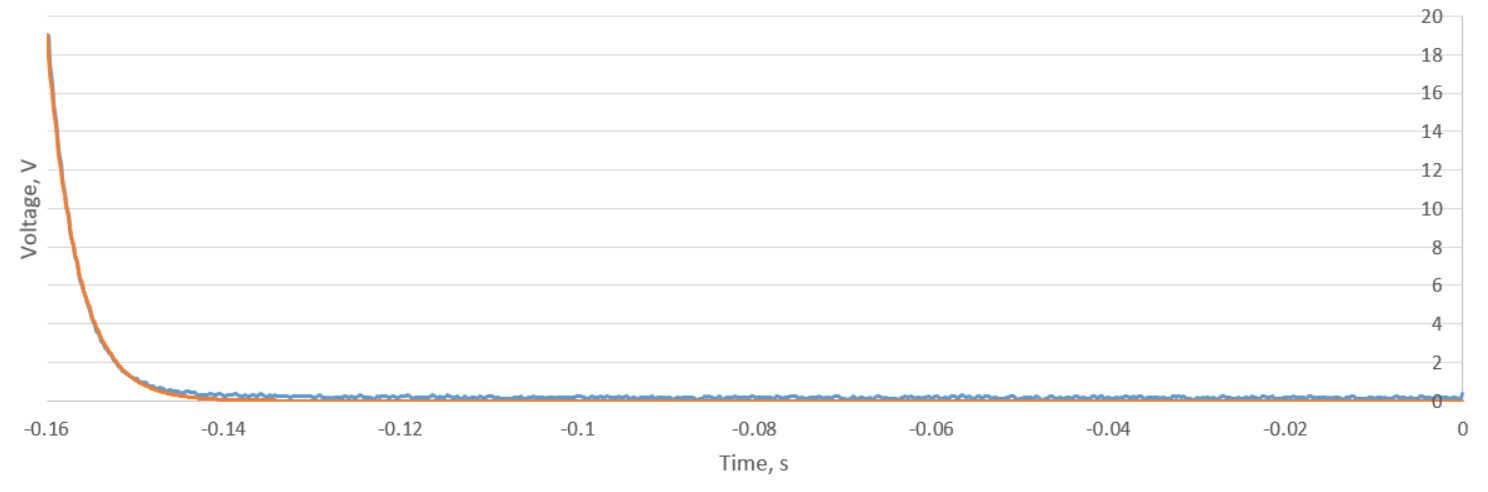
\includegraphics[width=0.65\linewidth]{figures/skew_quad_bcs/voltage_discharge_curve.png}
    \caption{Voltage discharge across the capacitor (in blue) with it \nth{1} order discharge fit (in orange)}
    \label{fig:resistor_voltage_discharge_curve}
\end{figure}

\begin{table}[h!]
    \caption{Heater characteristics} 
    \vspace{-1.em} 
    \fontsize{10}{10}
    \selectfont 
    \renewcommand{\arraystretch}{1.5}
    \begin{center}
    \begin{tabular}{ ccc }  
    \hline
    capacitance & 14 & [mF] \\
    time constant & 3.5 & [ms] \\
    heater resistance & 0.25 & [$\Omega$] \\
    \hline 
    \end{tabular}
    \end{center}  
     \label{table:heater_characteristics} 
 \end{table}

Assuming an adiabatic hot spot (no helium effect), one can deduce total energy input to the magnet as well as power input as a function of time. Power function can be easily deduced from the equation below. The power curve is presented in Fig. \ref{fig:hot_spot_power_input_curve}. After $t=10~\text{ms}$, the value of power is negligible, i.e. the capacitor is fully discharged.
\begin{equation}
    P(t) = \frac{1}{\text{dt}} (\frac{1}{2} \text{C}V^2)
\end{equation}

\begin{figure}[ht!]
    \centering
    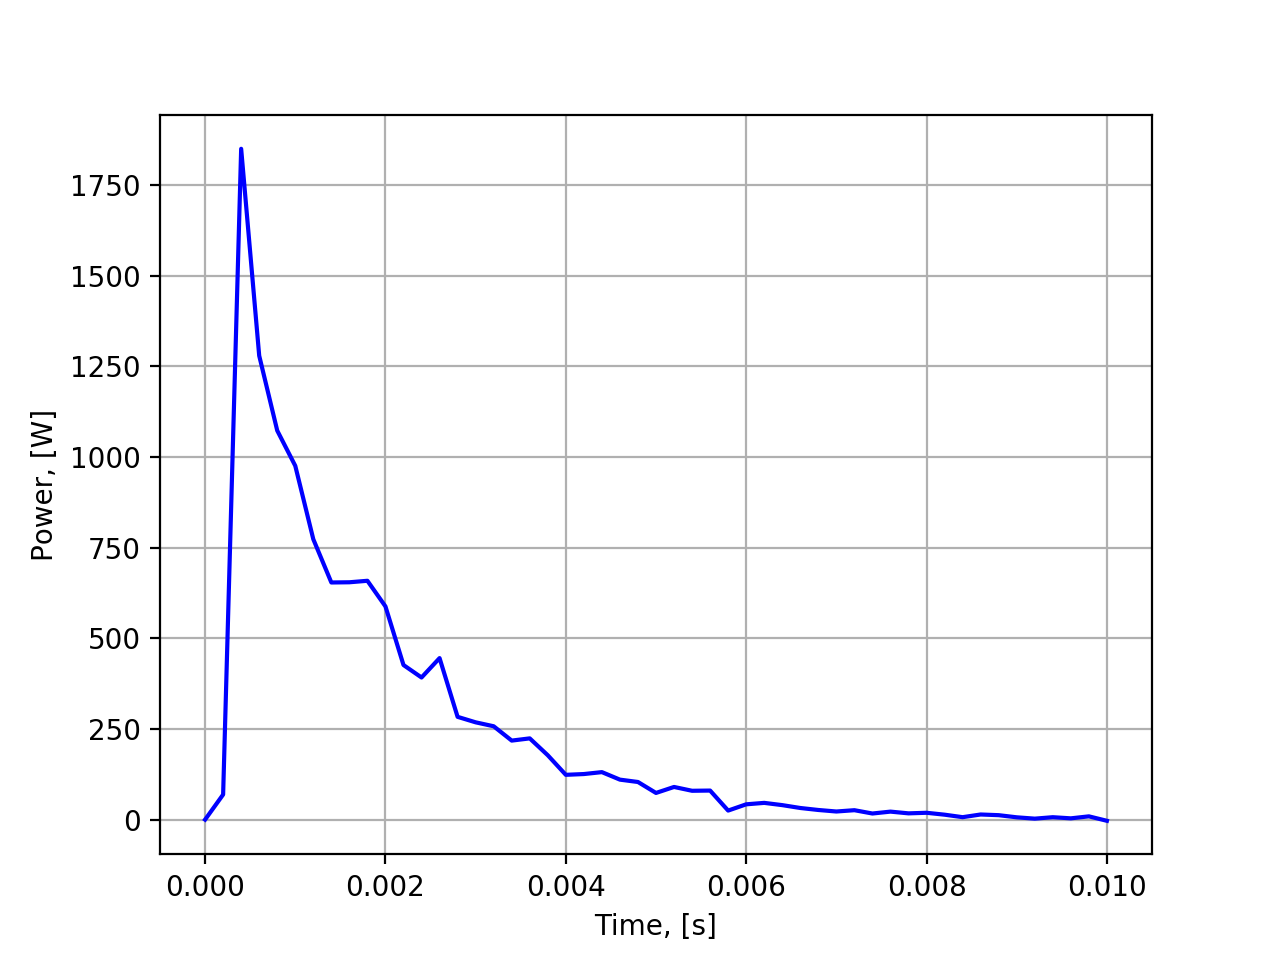
\includegraphics[width=0.45\linewidth]{figures/skew_quad_bcs/Polynomial_Power_Fit.png}
    \caption{Hot spot power input curve}
    \label{fig:hot_spot_power_input_curve}
\end{figure}

When the hot spot is applied, the individual windings start being normal conductive and, therefore resistive. The resistive voltage across the magnet increases, as presented in Fig. \ref{fig:res_volt_curve_quench_detection}. In skew quadrupole, the quench is detected if the magnet resistive voltage equal to at least $V=0.2~\text{V}$ last more than $t=20~\text{ms}$. At $t=0$, the power supply is cut off and the current starts decreasing.

\begin{figure}[ht!]
    \centering
    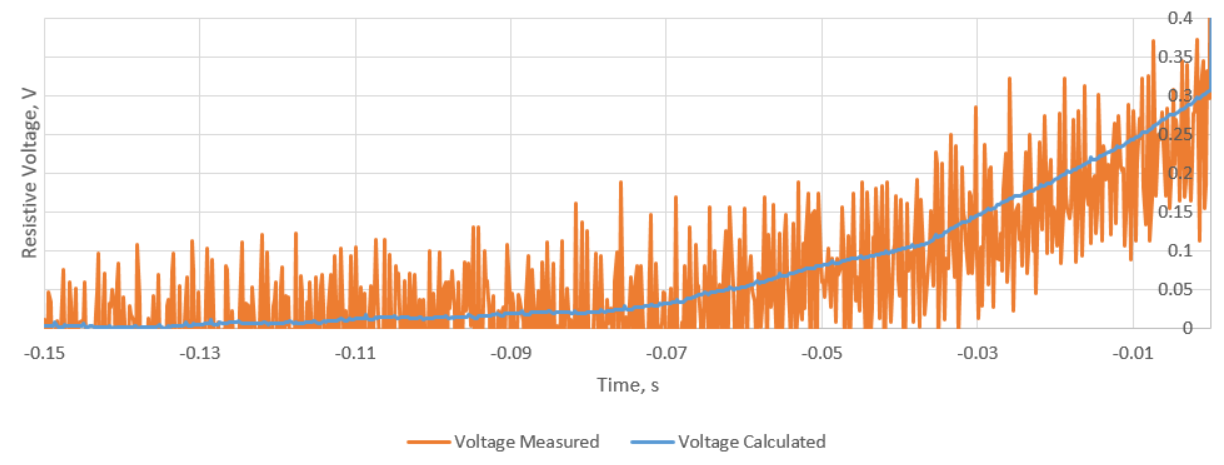
\includegraphics[width=0.6\linewidth]{figures/skew_quad_bcs/quench_det_v_curve.png}
    \caption{Resistive voltage rise until quench detection}
    \label{fig:res_volt_curve_quench_detection}
\end{figure}

\subsection{Magnetic Field Mapping}
Until the quench is detected, the current inside the magnet is constant and equal to $I=86~\text{A}$. Therefore, the magnetic field inside the magnet does not vary in time. The analysis of steady-state magnetic field in the middle of the magnet for this value of current was conducted at INFN-Milano in OPERA software \cite{samuele_mariotto_mails}. A 2D interpolation had to be conducted in order to fit the OPERA mesh with the windings' position. For each winding, it is assumed that it is subjected to the magnetic field from the centre of its cross-section estimated by the interpolation map presented in Fig. \ref{fig:Quad_Mag_contour1}.

\begin{figure}[ht!]
    \centering
    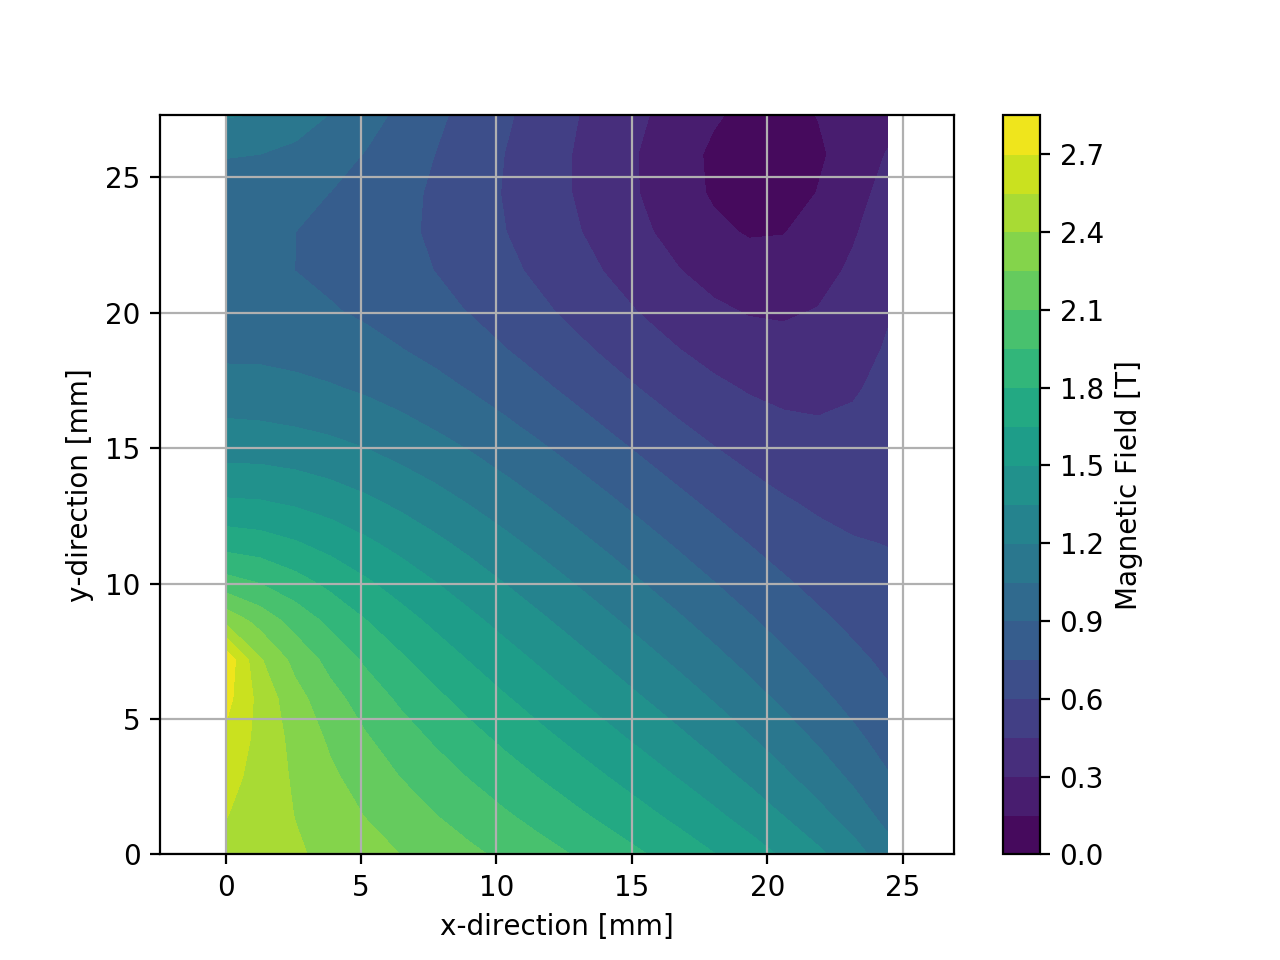
\includegraphics[width=0.49\linewidth]{figures/skew_quad_bcs/magnetic_field_mapping/Quadrupole_Magnetic_Colour_plot.png}
    \caption{Resultant magnetic field strength in the cross-section of skew quadrupole}
    \label{fig:Quad_Mag_contour1}
\end{figure}